\subsection{Supplementary Services}

As the other branches of the prototyping where happening, the need for additional services and infrastructure arose to 
support the development of the prototype as well as to increase the general usability of the prototype. 
This section will especially describe the services which help to make this prototype a more complete solution.


\begin{figure}[htb]
    \centering
    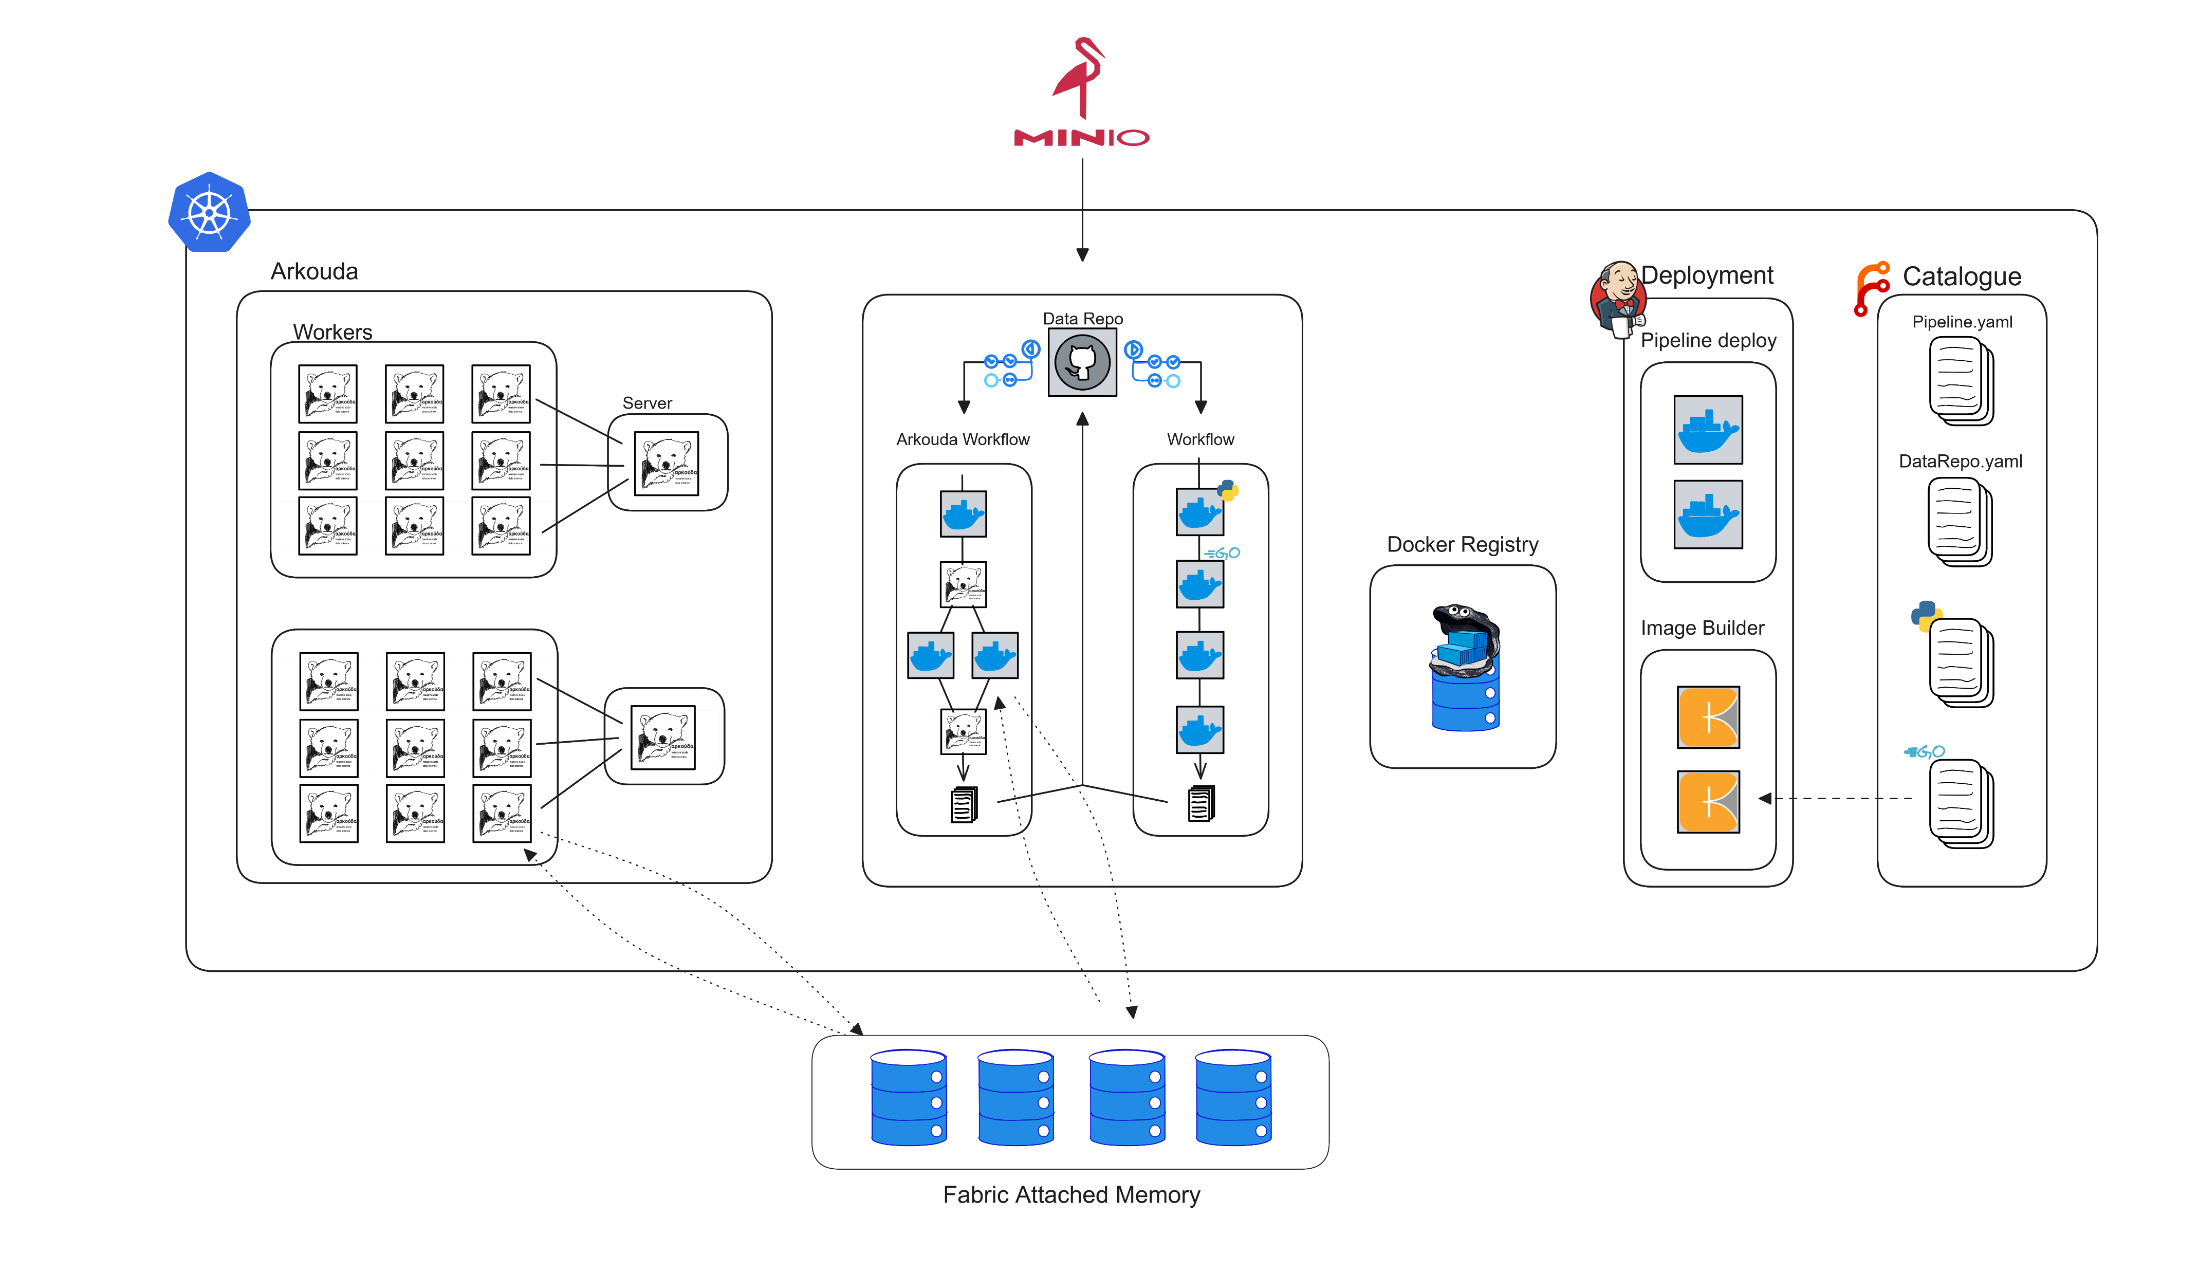
\includegraphics[width=17cm]{graphics/pachykouda_complete.png}
    \caption[Pachyderm High-Level Architecture]{Pachyderm High-Level Architecture}
    \label{abb:pachyderm_complete}
\end{figure}

\subsubsection{Docker Registry}

One thing that was quite apparent from the getgo, was the need for a central docker registry.
As Pachyderm does not manage the docker images itself, but relies on the user to provide them somehow externally.

During the first iterations when the development was being done on Minikube as described in \ref{minikube}, the internal Registry 
of the node was enough.
But as soon as we moved over to the Heydar system keeping the Hosts internal registries in sync was of course not feasible,
Therefore we added a private docker registry to the cluster \footcite{kumarHowSetupPrivate2020}.

\subsubsection{Frogejo Catalogue}
\subsubsection{Jenkins CI/CD Pipeline}
